% This file was created by tikzplotlib v0.9.2.
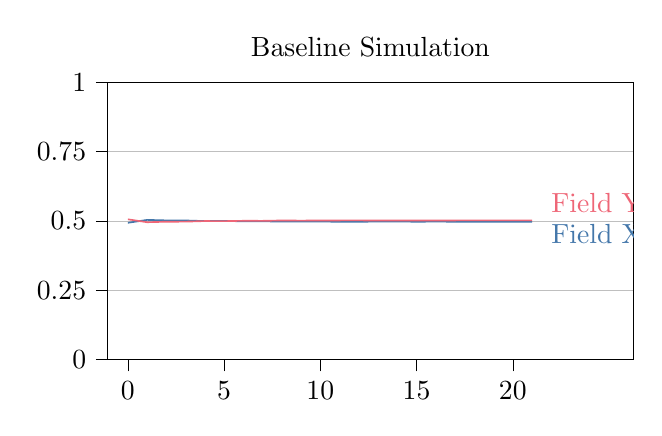
\begin{tikzpicture}

\definecolor{color0}{rgb}{0.266666666666667,0.466666666666667,0.666666666666667}
\definecolor{color1}{rgb}{0.933333333333333,0.4,0.466666666666667}

\begin{axis}[
height=5.101085673964669cm,
tick align=outside,
tick pos=left,
title={Baseline Simulation},
width=8.25373cm,
x grid style={white!69.0196078431373!black},
xmin=-1.05, xmax=26.25,
xtick style={color=black},
xtick={0,5,10,15,20},
xticklabels={\(\displaystyle 0\),\(\displaystyle 5\),\(\displaystyle 10\),\(\displaystyle 15\),\(\displaystyle 20\)},
ymajorgrids,
ymin=0, ymax=1,
ytick style={color=black},
ytick={0,0.25,0.5,0.75,1},
yticklabels={\(\displaystyle 0\),\(\displaystyle 0.25\),\(\displaystyle 0.5\),\(\displaystyle 0.75\),\(\displaystyle 1\)}
]
\addplot [semithick, color0]
table {%
0 0.4937
1 0.5042
2 0.5024
3 0.5021
4 0.5
5 0.5003
6 0.4991
7 0.4992
8 0.4979
9 0.4984
10 0.4979
11 0.4977
12 0.4976
13 0.498
14 0.498
15 0.4977
16 0.4979
17 0.4977
18 0.4976
19 0.4976
20 0.4976
21 0.4976
};
\addplot [semithick, color1]
table {%
0 0.5063
1 0.4958
2 0.4976
3 0.4979
4 0.5
5 0.4997
6 0.5009
7 0.5008
8 0.5021
9 0.5016
10 0.5021
11 0.5023
12 0.5024
13 0.502
14 0.502
15 0.5023
16 0.5021
17 0.5023
18 0.5024
19 0.5024
20 0.5024
21 0.5024
};
\draw (axis cs:21.5,0.4176) node[
  anchor=base west,
  text=color0,
  rotate=0.0
]{Field X};
\draw (axis cs:21.5,0.5324) node[
  anchor=base west,
  text=color1,
  rotate=0.0
]{Field Y};
\end{axis}

\end{tikzpicture}
